\subsubsection{Forward Backward Method}
The gradient shows the search direction and Fibonacci line search finds a minimizer to the one-dimensional problem contained within some bracket in this direction. It follows that some method for finding the bracket to contain the line search must be selected. For this purpose the forward backward method is chosen. The method attempts to find values of the cost function which goes from high to low to high.\\
The idea is simple, it takes a step forward from the initial point, evaluates the cost function, and if the value is higher than the original one it takes a step backward, otherwise it takes a step forward. If it finds high low low, the step-length is increased. Since it is searching in the gradient direction a low high high geometry indicates that the minimum lies in the found interval so long as the set searched is convex; that is, the initial step did not step over a peak of the performance function.\\
In \figref{gradientForwardBackwardAndFibonacci} an implementation of the gradient descend method is illustrated. \Figref{gradientForwardBackwardAndFibonacciZoom} shows how the gradient method generates a pattern with almost orthogonal lines converging to the minimum of the function.

\begin{minipage}{\linewidth}
	\begin{minipage}{0.45\linewidth}
		\begin{figure}[H]
			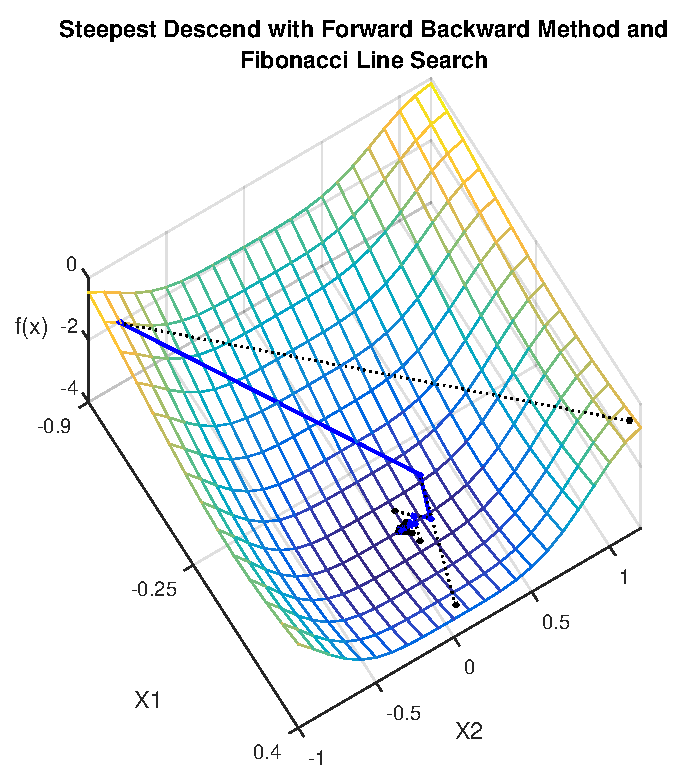
\includegraphics[scale=.6]{figures/gradientForwardBackwardAndFibonacci}
			\centering
			\captionsetup{justification=centering}
			\captionof{figure}{An example of a direct implementation of the gradient descend method using the forward backward method to determine the bracket in which the Fibonacci line search is used to solve each of the successive one-dimensional problems. The dotted lines represent the bracket found by the forward backward method in each iteration.}
			\label{gradientForwardBackwardAndFibonacci}
		\end{figure}
	\end{minipage}
	\hspace{0.03\linewidth}
	\begin{minipage}{0.45\linewidth}
		\begin{figure}[H]
			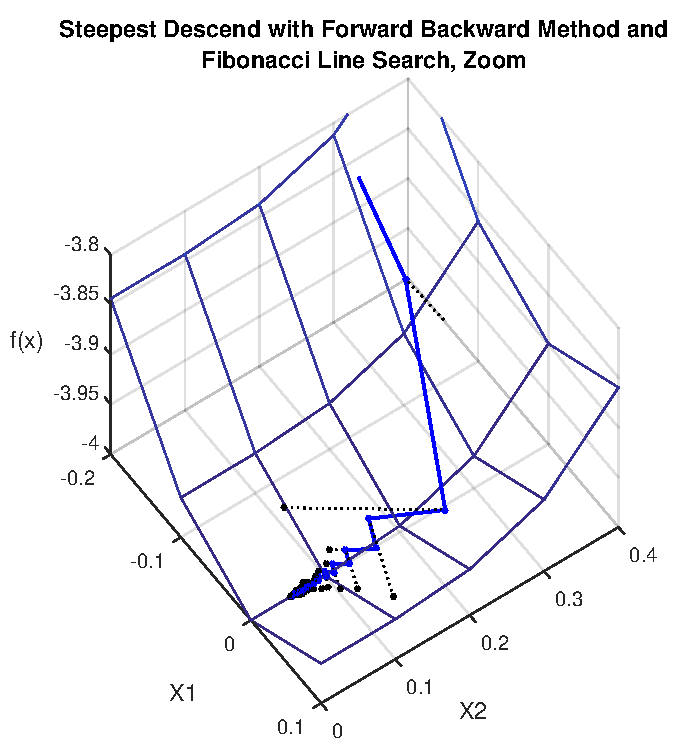
\includegraphics[scale=.62]{figures/gradientForwardBackwardAndFibonacciZoom}
			\centering
			\captionsetup{justification=centering}
			\captionof{figure}{Zoom on the convergence shows how the gradient descend method create a pattern with almost orthogonal lines converging to the minimum.\vspace{50pt}}
			\label{gradientForwardBackwardAndFibonacciZoom}
		\end{figure}
	\end{minipage}
\end{minipage}

With this background an implementation to solve the optimization problem presented in the beginning of this section described by \eqref{performanceFunction} has been done.

The result can be seen in \figref{paramEstFibonacci}, which gives \si{J_F=4,8 \cdot 10^{-3}\ kg \cdot m^2\ and\ B_F=7,8 \cdot 10^{-3}\ m \cdot s \cdot rad^{-1}}.

\begin{figure}[H]
	\centering
	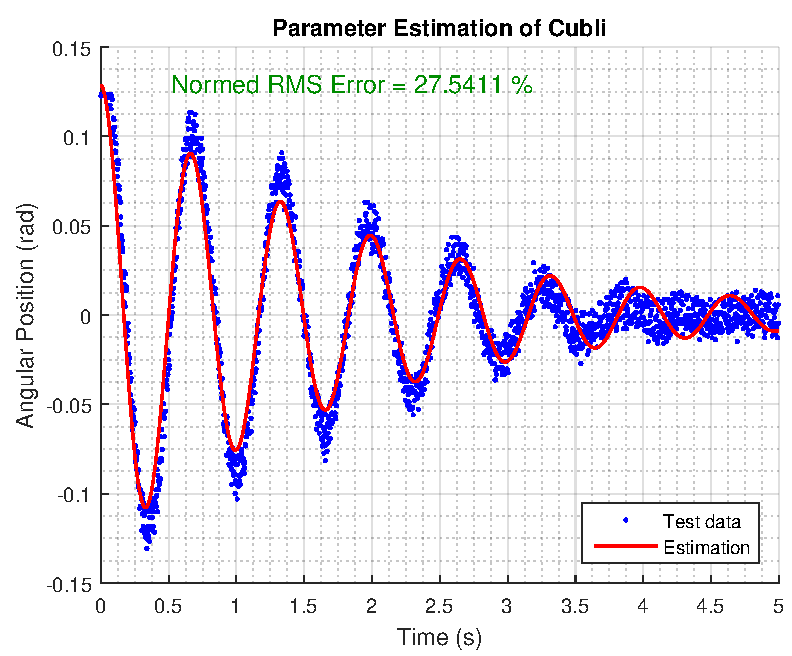
\includegraphics[scale=0.65]{figures/paramEstFibonacci}
	\caption{Data from the test (red) and final fit with the estimation of the parameters (blue)}
	\label{paramEstFibonacci}
\end{figure}